% A synthetic paper for the bare-number lint (tests/test_lint.py::test_the_corpus).
% It is no one's manuscript: it gathers the constructs real papers use around numbers
% that are not results. Exactly three typed numbers in it are results, marked SEEDED;
% the lint must flag those and nothing else. When a false positive is found in a real
% paper, add the construct here, with a comment saying what it is.
\documentclass[11pt,a4paper]{article}
\usepackage[margin=2.5cm,top=30mm]{geometry}
\usepackage{booktabs,amsmath,amsthm,graphicx,tikz,pgfplots,algorithm,algpseudocode,hyperref}
\usepackage{vouch}
\pgfplotsset{compat=1.18}
\setlength{\tabcolsep}{4pt}
\newcommand{\budget}{1200}
\declaretheorem[numberwithin=section]{theorem}
\definecolor{accent}{RGB}{31,119,180}

\begin{document}

\section{Results}
\label{sec:results12}

% a comment with 42 numbers in it, and 93.2 too
The classifier reaches \vouch{cifar.resnet.acc} on \vouch[,d]{cifar.n_images} images
(Figure~\ref{fig:curve}, Table~\ref{tab:main}, Eq.~\eqref{eq:loss}, and
\citep{Smith2020,Lee2024}). We follow the protocol of 2024, see
\url{https://example.org/data/12345} and \href{https://example.org/v/2}{version two}.

% SEEDED 1: a recorded value typed by hand (cifar.resnet.acc, 93.2%)
In words: it is right 93.2\% of the time.
% SEEDED 2: a recorded value typed by hand (cifar.n_images, 18,535)
It saw 18{,}535 images.
% SEEDED 3: a number no run produced
An earlier model reached 77.7\% here.

\begin{figure}[t]
\centering
\includegraphics[width=0.86\linewidth,trim=10 20 10 20,clip]{figures/curve}
\begin{tikzpicture}[scale=0.75, every node/.style={inner sep=2pt, minimum width=12mm}]
  \draw[thick, accent] (0,0) -- (12.5,0) -- (12.5,34);
  \node[anchor=west, xshift=12pt] at (3.25,1.5) {train};
  \foreach \x in {10,20,30} { \draw (\x/10,0) -- (\x/10,0.2); }
\end{tikzpicture}
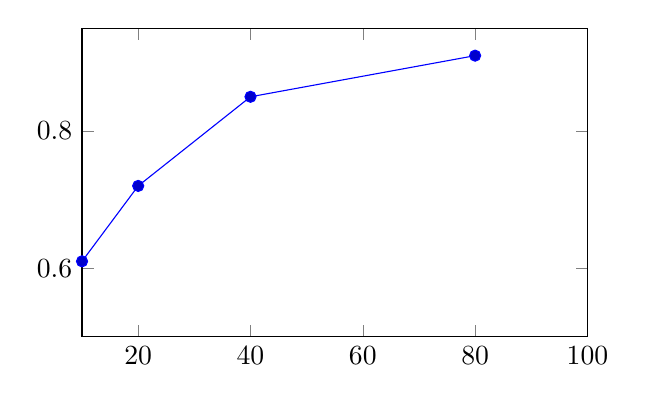
\begin{tikzpicture}
  \begin{axis}[xmin=10, xmax=100, ymin=0.5, ymax=0.95, width=8cm, height=55mm]
    \addplot coordinates {(10,0.61) (20,0.72) (40,0.85) (80,0.91)};
  \end{axis}
\end{tikzpicture}
\caption{Accuracy against epochs. \tikz\draw[accent] (0,0) -- (0.5,0); train,
\tikz\draw[dashed] (0,0) -- (0.5,0); test.}
\label{fig:curve}
\end{figure}

\begin{table}[t]
\centering
\begin{tabular}{@{}p{3.5cm}lrr@{}}
\toprule
model & data & accuracy & images \\[3pt]
\midrule
ResNet & CIFAR & \vouch{cifar.resnet.acc} & \vouch[,d]{cifar.n_images} \\
\bottomrule
\end{tabular}
\vspace{12pt}\hspace{0.5em}
\caption{The main result.}
\label{tab:main}
\end{table}

\begin{theorem}[Bound 3]
\label{thm:bound}
The error is at most $\epsilon^{2}/4$, and $n \geq 64$ suffices.
\end{theorem}

\begin{algorithm}[t]
\caption{Training}
\begin{algorithmic}[1]
\State $\eta \gets 10^{-3}$, $T \gets 100$
\For{$t = 1$ \textbf{to} $T$}
  \State update
\EndFor
\end{algorithmic}
\end{algorithm}

\begin{equation}
\mathcal L = \sum_{i=1}^{128} \ell_i
\label{eq:loss}
\end{equation}

\begin{verbatim}
python train.py --epochs 90 --lr 0.1
\end{verbatim}

\bibliographystyle{plain}
\bibliography{refs}
\end{document}
